\subsection{Chapter 16 - Gauss' Law}

\subsubsection{Overview}\label{chapter:gauss}

In this chapter, we take a detailed look at Gauss' law applied in the context of the electric field. We have already encountered Gauss' law briefly in Section {\textbackslash}ref\{sec:gravity:gauss\} when we examined the gravitational field. Since the electric force is mathematically identical to the gravitational force, we can apply the same tools, including Gauss' law, to model the electric field as we do the gravitational field. Many of the results from this chapter are thus equally applicable to the gravitational force.

\begin{framed}
\textbf{Learning Objectives}\\
\begin{itemize}
\item Understand the concept of flux for a vector field.
\item Understand how to calculate the flux of a vector field through an open and a closed surface.
\item Understand how to apply Gauss' law quantitatively to determine an electric field.
\item Understand how to apply Gauss' law qualitatively to discuss charges on a conductor.
\end{itemize}
\end{framed}

\begin{framed}
\textbf{Think About It}\\
A neutral spherical conducting shell encloses a point charge, $Q$, located at the centre of the shell. Due to separation of charge, the outer surface of the shell will acquire a net positive charge. What is the magnitude of that charge? \}

\begin{enumerate}
\item less than $Q$.
\item exactly $Q$.
\item more than $Q$.
\end{enumerate}

\begin{framed}
\textbf{Answer}\\
\begin{enumerate}[resume]
\item
\end{enumerate}
\end{framed}
\end{framed}

\subsubsection{Flux of the electric field}\label{sec:gauss:flux}

Gauss' law makes use of the concept of ``flux''. Flux is always defined based on:

\begin{enumerate}
\item A surface.
\item A vector field (e.g. the electric field).
\end{enumerate}

and can be thought of as a measure of the number of field lines from the vector field that cross the given surface. For that reason, one usually refers to the ``flux of the electric field through a surface''. This is illustrated in Figure~\ref{fig:gauss:fluxangle} for a uniform horizontal electric field, and a flat surface, whose normal vector, $\vec A$, is shown. If the surface is perpendicular to the field (left panel), so that the field vector is parallel to $\vec A$, then the flux through that surface is maximal. If the surface is parallel to the field (right panel), then no field lines cross that surface, and the flux through that surface is zero. If the surface is rotated with respect to the electric field, as in the middle panel, then the flux through the surface is between zero and the maximal value.

\begin{figure}[!htbp]
\centering
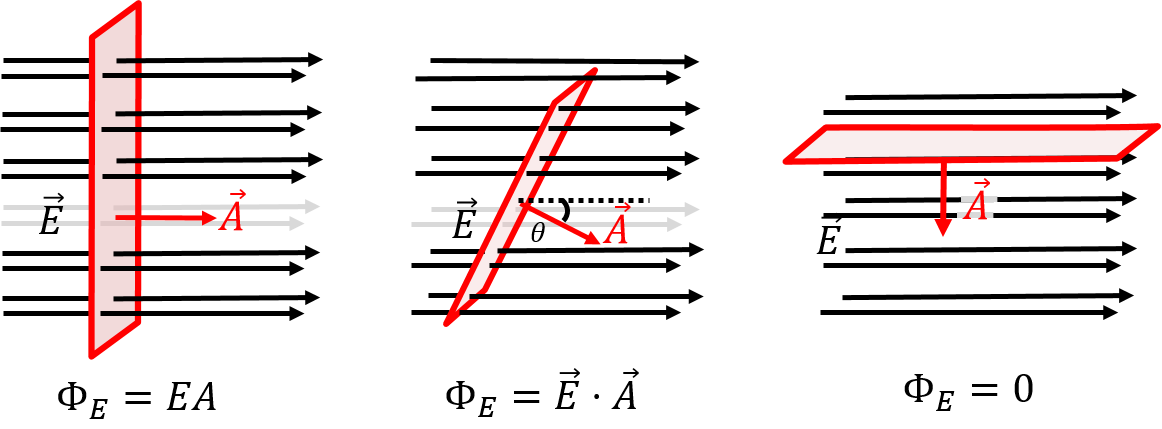
\includegraphics[width=0.9\linewidth]{files/fluxangle-958ab1f9963cf42848c577cd247fa3d9.png}
\caption[]{Flux of an electric field through a surface that makes different angles with respect to the electric field. In the leftmost panel, the surface is oriented such that the flux through it is maximal. In the rightmost panel, there are no field lines crossing the surface, so the flux through the surface is zero.}
\label{fig:gauss:fluxangle}
\end{figure}

The vector $\vec A$ is used to represent the surface. It is defined so that the magnitude of $\vec A$ is equal to the area of the surface and the direction of $\vec A$ is perpendicular to the surface, as illustrated in Figure~\ref{fig:gauss:fluxangle}. We define the flux, $\Phi_E$, of the electric field, $\vec E$, through the surface represented by vector $\vec A$ as:
\begin{equation}
\Phi_E=\vec E\cdot \vec A=EA\cos\theta
\end{equation}
since this will have the same properties that we described above (e.g. the flux is zero when $\vec E$ and $\vec A$ are perpendicular, and the flux is proportional to number of field lines crossing the surface). Note that, because we only require that $\vec A$ is perpendicular to the surface, there are two possible choices for the direction of $\vec A$. As a result, the flux could be either positive or negative. By convention, we usually choose $\vec A$ so that the flux is positive.

\begin{framed}
\textbf{Olivia's Thoughts}\\
In the most general terms, flux is the amount of something passing through an area. In the case of the electric flux, this is the number of electric field lines passing through a surface. We can draw parallels between the electric flux and a more intuitive example of flux: the amount of water flowing through a net. Imagine submerging a net in a flowing river. The amount of water that flows through the net will depend on the strength of the current (this is like $E$), the orientation of the net relative to the flow of water ($\cos\theta$), and the size of the net ($A$). When trying to conceptualize problems about electric flux, it sometimes helps to think of the field lines as representing water currents and the surface as representing a net in order to visualize what's going on in the problem.
\end{framed}

\begin{framed}
\textbf{Checkpoint}\\
What are the S.I. units of electric flux?

\begin{enumerate}
\item ${\rm N\cdot m/C}$
\item ${\rm V\cdot m}$
\item ${\rm V/m}$
\item The units of flux depend on the dimensions of the charged object.
\end{enumerate}

\begin{framed}
\textbf{Answer}\\
\begin{enumerate}[resume]
\item
\end{enumerate}
\end{framed}
\end{framed}

\begin{framed}
\textbf{Example 16.1}\\
A uniform electric field is given by: $\vec E=E\cos\theta~\hat x+E\sin\theta~\hat y$ throughout space. A rectangular surface is defined by the four points $(0,0,0)$, $(0,0,H)$, $(L,0,0)$, $(L,0,H)$. What is the flux of the electric field through the surface?

\begin{framed}
\textbf{Solution}\\
The surface that is defined corresponds to a rectangle in the $xz$ plane with area $A=LH$. Since the rectangle lies in the $xz$ plane, a vector perpendicular to the surface will be along the $y$ direction. We choose the positive $y$ direction, since this will give a positive number for the flux (as the electric field has a positive component in the $y$ direction). The vector $\vec A$ is given by:
\begin{equation}
\vec A =A\hat y=LH\hat y
\end{equation}
The flux through the surface is thus given by:
\begin{equation}
\Phi_E&=\vec E\cdot \vec A=(E\cos\theta\hat x+E\sin\theta\hat y)\cdot(LH\hat y)\\
&=ELH\sin\theta
\end{equation}
where one should note that the angle $\theta$, in this case, is not the angle between $\vec E$ and $\vec A$, but rather the complement of that angle.

\textbf{Discussion:} In this example, we calculated the flux of a uniform electric field through a rectangle of area, $A=LH$. Since we knew the components of both the electric field vector, $\vec E$, and the surface vector, $\vec A$, we used their scalar product to determine the flux through the surface. In some cases, it is easier to work with the magnitude of the vectors and the angle between them to determine the scalar product (although note that in this example, the angle between $\vec E$ and $\vec A$ is $90{\degree} -\theta$).
\end{framed}
\end{framed}

\paragraph{Non-uniform fields}

So far, we have considered the flux of a uniform electric field, $\vec E$, through a surface, $S$, described by a vector, $\vec A$. In this case, the flux, $\Phi_E$, is given by:
\begin{equation}
\Phi_E=\vec E\cdot \vec A
\end{equation}
However, if the electric field is not constant in magnitude and/or in direction over the entire surface, then we divide the surface, $S$, into many infinitesimal surfaces, $dS$, and sum together (integrate) the fluxes from those infinitesimal surfaces:
\begin{equation}
\boxed{\Phi_E=\int \vec E\cdot d\vec A}
\end{equation}
where, $d\vec A$, is the normal vector for the infinitesimal surface, $dS$. This is illustrated in Figure~\ref{fig:gauss:fluxdA}, which shows, in the left panel, a surface for which the electric field changes magnitude along the surface (as the field lines are closer in the lower left part of the surface), and, in the right panel, a scenario in which the direction and magnitude of the electric field vary along the surface.

In order to calculate the flux through the total surface, we first calculate the flux through an infinitesimal surface, $dS$, over which we assume that $\vec E$ is constant in magnitude and direction, and then, we sum (integrate) the fluxes from all of the infinitesimal surfaces together. Remember, the flux through a surface is related to the number of field lines that cross that surface; it thus makes sense to count the lines crossing an infinitesimal surface, $dS$, and then adding those together over all the infinitesimals surfaces to determine the flux through the total surface, $S$.

\begin{figure}[!htbp]
\centering
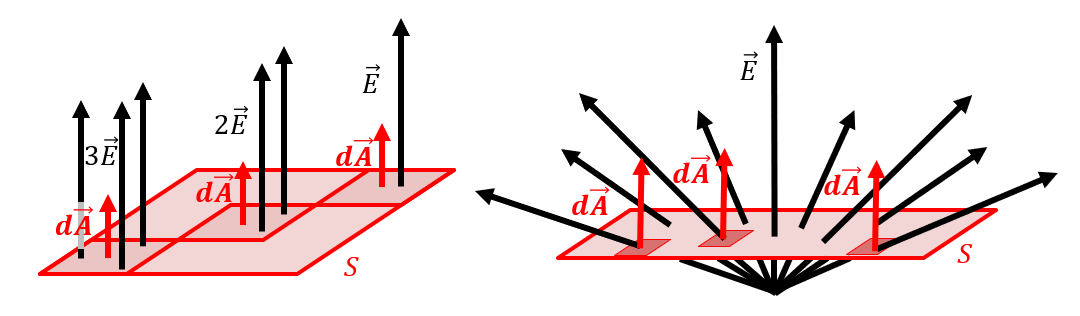
\includegraphics[width=0.9\linewidth]{files/fluxdA-675e21c7412f32ffebdb6ac667e6b1ef.png}
\caption[]{Examples of surfaces that need to be sub-divided in order to determine the net flux through them. The surface on the left must be subdivided because the electric field changes magnitude over the surface, whereas the one on the right needs to be subdivided because the angle between $\vec E$ and $d\vec A$ is not constant (and the magnitude of $\vec E$ also changes along the surface).}
\label{fig:gauss:fluxdA}
\end{figure}

\begin{framed}
\textbf{Example 16.2}\\
An electric field points in the $z$ direction everywhere in space. The magnitude of the electric field depends linearly on the $x$ position in space, so that the electric field vector is given by: $\vec E=(ax -b)\hat z$, where $a$ and $b$ are constants. What is the flux of the electric field through a square with side length $L$ that is located in the positive $xy$ plane with one of its corners at the origin?

\begin{framed}
\textbf{Solution}\\
We need to calculate the flux of the electric field through a square of side length $L$ in the $xy$ plane. The electric field is always in the $z$ direction, so the angle between $\vec E$ and $d\vec A$ (the normal vector for any infinitesimal area element) will remain constant. We can calculate the flux through the square by dividing up the square into thin strips of length $L$ in the $y$ direction and infinitesimal width $dx$ in the $x$ direction, as illustrated in Figure~\ref{fig:gauss:fluxlinx}. We can do this because the electric field does not change with $y$, so the flux along each of these strips will be constant. If the electric field varied both as a function of $x$ and $y$, we would start with area elements that have infinitesimal dimensions in both the $x$ and the $y$ directions.

\begin{figure}[!htbp]
\centering
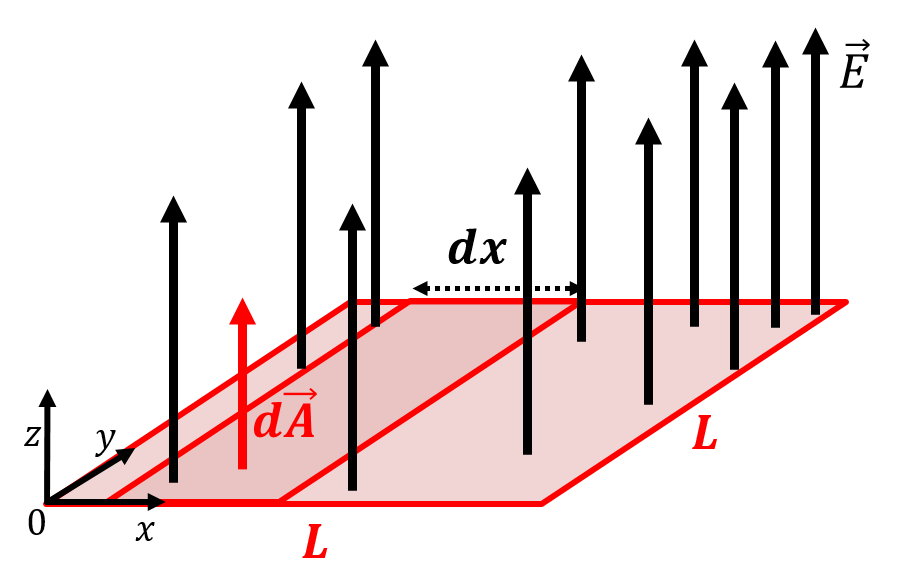
\includegraphics[width=0.5\linewidth]{files/fluxlinx-e8e921d01654ee11a768fd94b9df938c.png}
\caption[]{Dividing a square in the $xy$ plane into thin strips of length $L$ and width $dx$.}
\label{fig:gauss:fluxlinx}
\end{figure}

As illustrated in Figure~\ref{fig:gauss:fluxlinx}, we first calculate the flux through a thin strip of area, $dA=Ldx$, located at position $x$ along the $x$ axis. Choosing the direction of $d\vec A$ so that it gives a positive flux, we can obtain the flux through the strip:
\begin{equation}
d\Phi_E=\vec E\cdot d\vec A=EdA=(ax-b)Ldx
\end{equation}
where $\vec E\cdot d\vec A=EdA$, since the angle between $\vec E$ and $\vec A$ is zero. Summing together the fluxes from the strips, from $x=0$ to $x=L$, the total flux is given by:
\begin{equation}
\Phi_E=\int d\Phi_E=\int_0^L(ax-b)Ldx=\frac{1}{2}aL^3-bL^2
\end{equation}
\textbf{Discussion:} In this example, we showed how to calculate the flux from an electric field that changes magnitude with position. We modelled a square of side length $L$ as being made of many thin strips of length $L$ and width $dx$. We then calculated the flux through each strip and added those together to obtain the total flux through the square.
\end{framed}
\end{framed}

\paragraph{Closed surfaces}\label{sec:gauss:closedsurfaces}

One can distinguish between a ``closed'' surface and an ``open'' surface. A surface is closed if it completely defines a volume that could, for example, be filled with a liquid.  A closed surface has a clear ``inside'' and an ``outside''. For example, the surface of a sphere, of a cube, or of a cylinder are all examples of closed surfaces. A plane, a triangle, and a disk are, on the other hand, examples of ``open surfaces''.

For a closed surface, one can unambiguously define the direction of the vector $\vec A$ (or $d\vec A$) as the direction that it is perpendicular to the surface and \textbf{points towards the outside}. Thus, the sign of the flux out of a closed surface is meaningful. The flux will be positive if there is a net number of field lines exiting the volume defined by the surface (since $\vec E$ and $\vec A$ will be parallel on average) and the flux will be negative if there is a net number of field lines entering the volume (as $\vec E$ and $\vec A$ will be anti-parallel on average). The flux through a closed surface is thus zero if the number of field lines that enter the surface is the same as the number of field lines that exit the surface. When calculating the flux over a closed surface, we use a different integration symbol to show that the surface is closed:
\begin{equation}
\Phi_E=\oint \vec E\cdot d\vec A
\end{equation}
which is the same integration symbol that we used for indicating a path integral when the initial and final points are the same (see, for example, Section~\ref{sec:potentialecons:conservative}).

\begin{framed}
\textbf{Checkpoint}\\
\begin{figure}[!htbp]
\centering
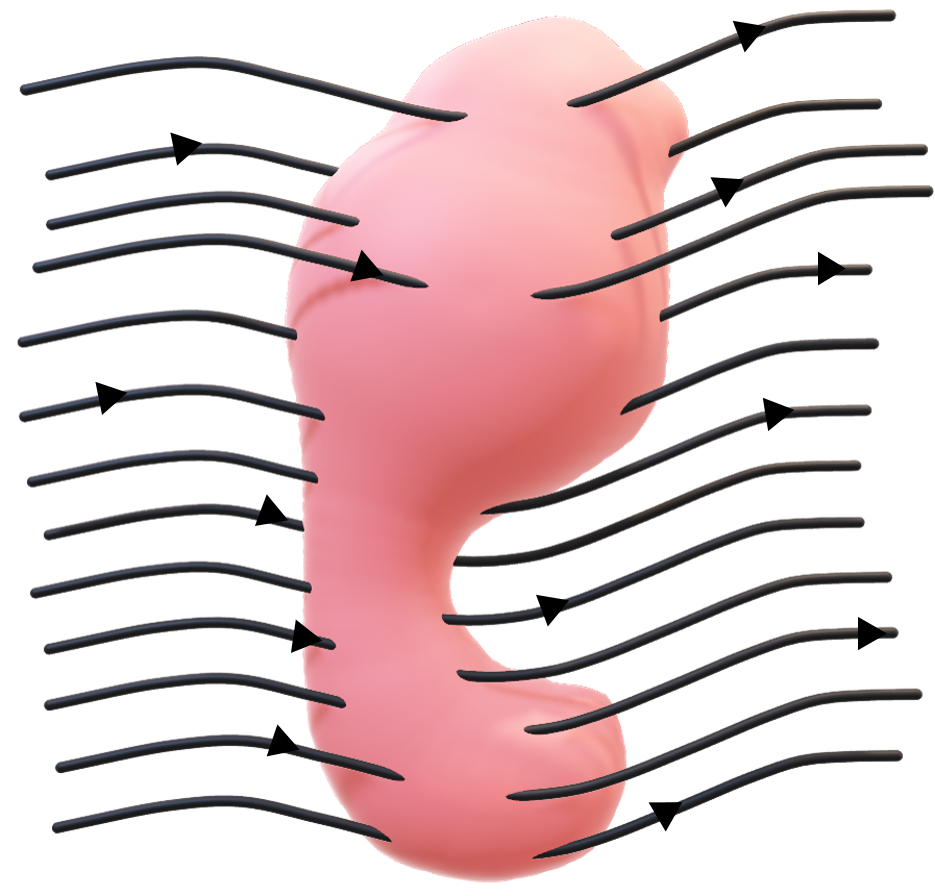
\includegraphics[width=0.25\linewidth]{files/irregularfield-0ce5dc8f672cf41596e1d051d4a15239.png}
\caption[]{A non-uniform electric field flowing through an irregularly shaped closed surface.}
\label{fig:gauss:irregularfield}
\end{figure}

A non-uniform electric field $\vec E$ flows through an irregularly-shaped closed surface, as shown in Figure~\ref{fig:gauss:irregularfield}. The flux through the surface is

\begin{enumerate}
\item positive.
\item zero.
\item negative.
\end{enumerate}

\begin{framed}
\textbf{Answer}\\
\begin{enumerate}[resume]
\item
\end{enumerate}
\end{framed}
\end{framed}

\begin{framed}
\textbf{Olivia's Thoughts}\\
Consider the water flowing through a net analogy again, although now the net is a closed surface (e.g. a sphere). If there is more water flowing out of the net than into it, the flux is positive. If there is more flowing in than out, the flux is negative. If there is an equal amount of water flowing in and out, the flux is zero. If you had trouble with the last checkpoint question, try it again but now thinking about the field lines as a flow of water. Is there more water flowing in or out of the object, or is it the same?
\end{framed}

\begin{framed}
\textbf{Example 16.3}\\
A negative electric charge, $-Q$, is located at the origin of a coordinate system. Calculate the flux of the electric field through a spherical surface of radius, $R$, that is centred at the origin.

\begin{framed}
\textbf{Solution}\\
Figure~\ref{fig:gauss:fluxsphere} shows the spherical surface of radius, $R$, centred on the origin where the charge $-Q$ is located.

\begin{figure}[!htbp]
\centering
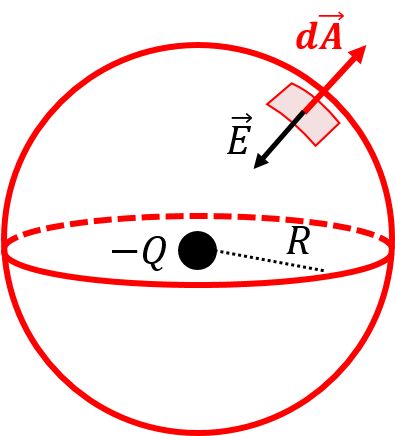
\includegraphics[width=0.3\linewidth]{files/fluxsphere-ae8a21173bcf1a55fdaa3f4d3992daec.png}
\caption[]{Calculating the flux through a spherical surface.}
\label{fig:gauss:fluxsphere}
\end{figure}

At all points along the surface, the electric field has the same magnitude:
\begin{equation}
E=\frac{1}{4\pi\epsilon_0}\frac{Q}{R^2}
\end{equation}
as given by Coulomb's law for a point charge. Although the vector $\vec E$ changes direction everywhere along the surface, it always makes the same angle ({\textbackslash}SI\{-180\}\{{\textbackslash}degree\}) with the corresponding vector $d\vec A$ at any particular location. Indeed, for a point charge, the electric field points in the radial direction (inwards for a negative charge) and is thus perpendicular to the spherical surface at all points. Since the surface is closed, the vector $d\vec A$ points outwards anywhere on the surface. Thus, at any point on the surface, we can evaluate the flux through an infinitesimal area element, $d\vec A$:
\begin{equation}
d\Phi_E=\vec E\cdot d\vec A=EdA\cos(-180\degree)=-EdA
\end{equation}
where the overall minus sign comes from the fact that $\vec E$ and $d\vec A$ are anti-parallel. The total flux through the spherical surface is obtained by summing together the fluxes through each area element:
\begin{equation}
\Phi_E=\oint d\Phi_E=\oint -EdA=-E\oint dA=-E(4\pi R^2)
\end{equation}
where we factored $E$ out of the integral, since the magnitude of the electric field is constant over the entire surface (a constant distance $R$ from the charge). In the last equality, we recognized that, $\oint dA$, simply means ``sum together all of the areas, $dA$, of the surface elements'', which gives the total surface area of the sphere, $4\pi R^2$. The flux through the spherical surface is negative, because the charge is negative, and the field lines point towards $-Q$.

Using the value that we obtained for the magnitude of the electric field from Coulomb's Law, the total flux is given by:
\begin{equation}
\Phi_E=-E(4\pi R^2)=-\frac{1}{4\pi\epsilon_0}\frac{Q}{R^2}(4\pi R^2)=-\frac{Q}{\epsilon_0}
\end{equation}
which, surprisingly, is independent of the radius of the spherical surface. Note that we used $\epsilon_0$ instead of Coulomb's constant, $k$, since the result is cleaner without the extra factor of $4\pi$.

\textbf{Discussion:} In this example, we calculated the flux of the electric field from a negative point charge through a spherical surface concentric with the charge. We found the flux to be negative, which makes sense, since the field lines go towards a negative charge, and there is thus a net number of field lines entering the spherical surface. Perhaps surprisingly, we found that the total flux through the surface does not depend on the radius of the surface! In fact, that statement is precisely Gauss' law: the net flux out of a closed surface depends only on the amount of charge enclosed by that surface (and the constant, $\epsilon_0$). Gauss' law is of course more general, and applies to surfaces of any shape, as well as charges of any shape (whereas Coulomb's Law only holds for point charges).
\end{framed}
\end{framed}

\subsubsection{Gauss' Law}

Gauss' law is a relation between the net flux through a closed surface and the amount of charge, $Q^{enc}$, in the volume enclosed by that surface:
\begin{equation}
\boxed{\oint \vec E\cdot d\vec A=\frac{Q^{enc}}{\epsilon_0}}
\end{equation}
In particular, note that Gauss' law holds true for \textbf{any} closed surface, and the shape of that surface is not specified in Gauss' law.  That is, we \textbf{can always choose the surface to use} when calculating the flux. For obvious reasons, we often call the surface that we choose a ``Gaussian surface''. But again, this surface is simply a mathematical tool, there is no actual property that makes a surface ``Gaussian''; it simply means that we chose that surface in order to apply Gauss' law.  In Example~16.3 above, we confirmed that Gauss' law is compatible with Coulomb's Law for the case of a point charge and a spherical Gaussian surface.

Physically, Gauss' law is a statement that field lines must begin or end on a charge (electric field lines originate on positive charges and terminate on negative charges). Recall, flux is a measure of the net number of lines coming out of a surface. If there is a net number of lines coming out of a closed surface (a positive flux), that surface must enclose a positive charge from where those field lines originate. Similarly, if there are the same number of field lines entering a closed surface as there are lines exiting that surface (a flux of zero), then the surface encloses no charge. Gauss' law simply states that the number of field lines exiting a closed surface is proportional to the amount of charge enclosed by that surface.

Primarily, Gauss' law is a useful tool to determine the magnitude of the electric field from a given charge, or charge distribution. We usually have to use symmetry to determine the direction of the electric field vector. In general, the integral for the flux is difficult to evaluate, and Gauss' law can only be used analytically in cases with a high degree of symmetry. Specifically, the integral for the flux is easiest to evaluate if:

\begin{enumerate}
\item \textbf{The electric field makes a constant angle with the surface}. When this is the case, the scalar product can be written in terms of the cosine of the angle between $\vec E$ and $d\vec A$, which can be taken out of the integral if it is constant:
\end{enumerate}
\begin{equation}
\oint \vec E\cdot d\vec A=\oint E\cos\theta dA=\cos\theta\oint EdA
\end{equation}
Ideally, one has chosen a surface such that this angle is 0 or $180\degree$.

\begin{enumerate}[resume]
\item \textbf{The electric field is constant in magnitude along the surface}. When this is the case, the integral can be simplified further by factoring out $E$ and simply becomes an integral over $dA$ (which corresponds to the total area of the surface, $A$):
\end{enumerate}
\begin{equation}
\oint \vec E\cdot d\vec A=\cos\theta\oint EdA =E\cos\theta\oint dA=EA\cos\theta
\end{equation}
Ultimately, the points above should dictate the choice of Gaussian surface \textbf{so that} the integral for the flux is easy to evaluate. The choice of surface will depend on the symmetry of the problem. For a point (or spherical) charge, a spherical Gaussian surface allows the flux to easily be calculated (Example~16.3). For a line of charge, as we will see, a cylindrical surface results is a good choice for the Gaussian surface. Broadly, the steps for applying Gauss' law to determine the electric field are as follows:

\begin{enumerate}
\item Make a diagram showing the charge distribution.
\item Use symmetry arguments to determine in which way the electric field vector points.
\item Choose a Gaussian surface that goes through the point for which you want to know the electric field. Ideally, the surface is such that the electric field is constant in magnitude and always makes the same angle with the surface, so that the flux integral is straightforward to evaluate.
\item Calculate the flux, $\oint \vec E\cdot d\vec A$.
\item Calculate the amount of charge located within the volume enclosed by the surface, $Q^{enc}$.
\item Apply Gauss' law,  $\oint \vec E\cdot d\vec A=\frac{Q^{enc}}{\epsilon_0}$.
\end{enumerate}

\begin{framed}
\textbf{Example 16.4}\\
An insulating sphere of radius, $R$, contains a total charge, $Q$, which is uniformly distributed throughout its volume. Determine an expression for the electric field as a function of distance, $r$, from the centre of the sphere.
Note that this is identical, mathematically, to the derivation that was done in Section~\ref{sec:gravity:gauss} for the case of gravity.

\begin{framed}
\textbf{Solution}\\
When applying Gauss' law,  we first need to think about symmetry in order to determine the direction of the electric field vector. We also need to think about all possible regions of space in which we need to determine the electric field. In particular, for this case, we need to determine the electric field both inside ($r\leq R$) and outside ($r\geq R$) of the charged sphere.

Figure~\ref{fig:gauss:spheresymmetry} shows the charged sphere of radius $R$. If we consider the direction of the electric field outside the sphere (where $\vec E_{out}$ is drawn), we realize that it can only point in the radial direction (towards or away from the centre of the sphere), as this is the only choice that preserves the symmetry of the sphere. Being a sphere, the charge looks the same from all angles; thus, the electric field must also look the same from all angles, otherwise, there would be a preferred orientation for the sphere. The same argument holds for the electric field vector inside the sphere (drawn as $\vec E_{in}$).

\begin{figure}[!htbp]
\centering
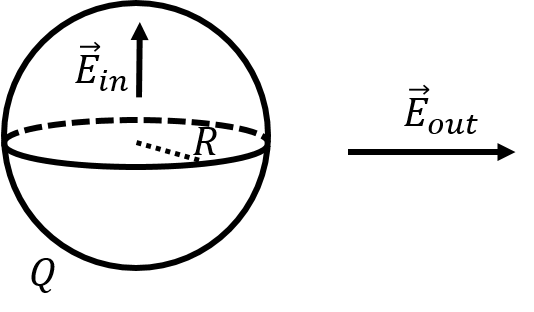
\includegraphics[width=0.4\linewidth]{files/spheresymmetry-cfcd411403bc4dc5e77a998a9afcd219.png}
\caption[]{For a spherical charge distribution, the electric field inside and outside must point in the radial direction, by symmetry.}
\label{fig:gauss:spheresymmetry}
\end{figure}

We now need to choose a Gaussian surface that will make the flux integral easy to evaluate. Ideally, we can find a surface over which the electric field makes the same angle with the surface and over which the electric field is constant in magnitude. Again, based on the symmetry of the charge distribution, it is clear that a spherical surface of radius, $r$, will satisfy these properties.

We start by applying Gauss' law outside the charge (with $r\geq R$) to determine the electric field, $\vec E_{out}$. Figure~\ref{fig:gauss:spherein} shows our choice of spherical Gaussian surface (labelled $S$) of radius, $r$, which is concentric with the spherical charge distribution of radius, $R$, and total charge, $+Q$.

\begin{figure}[!htbp]
\centering
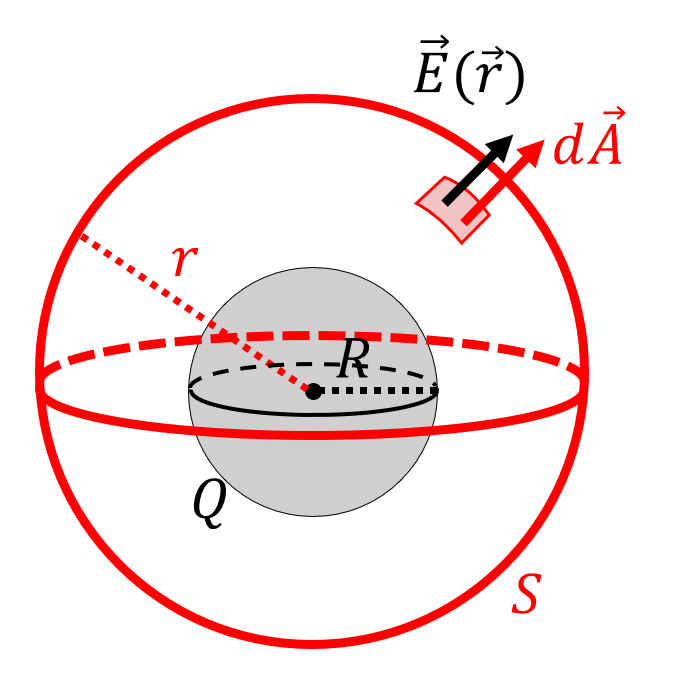
\includegraphics[width=0.4\linewidth]{files/spherein-1460112cc9e975744df1cf30fe343f7c.png}
\caption[]{A spherical Gaussian surface to determine the electric field outside of a sphere of radius, $R$, holding charge, $+Q$.}
\label{fig:gauss:spherein}
\end{figure}

In order to apply Gauss' law,  we need to calculate:

\begin{itemize}
\item the net flux through the surface.
\item the charge in the volume enclosed by the surface.
\end{itemize}

The net flux through the surface is found in the same way as in Example~16.3, and is given by:
\begin{equation}
\Phi_E&=\oint \vec E\cdot d\vec A=\oint E dA= E\oint dA=E(4\pi r^2)
\end{equation}
where our choice of spherical surface led to $\vec E\cdot d\vec A=EdA$, since $\vec E$ and $d\vec A$ are always parallel. Furthermore, by symmetry, the electric field must be constant in magnitude along the whole surface, or the spherical symmetry would be broken. This allowed us to factor the $E$ out of the integral, leaving us with, $\oint dA$, which is simply the area of our Gaussian spherical surface, $4\pi r^2$.

The Gaussian surface with $r\geq R$ encloses the whole charged sphere, so the charge enclosed is simply the charge of the sphere, $Q^{enc}=Q$. Applying Gauss' law allows us to determine the magnitude of the electric field:
\begin{equation}
\oint \vec E\cdot d\vec A&=\frac{Q^{enc}}{\epsilon_0} \\
E(4\pi r^2) &= \frac{Q}{\epsilon_0}\\
\therefore E&= \frac{1}{4\pi\epsilon_0}\frac{Q}{r^2}
\end{equation}
which is the same as the electric field a distance $r$ from a point charge. Thus, from the outside, a spherical charge distribution leads to the same electric field as if the charge were concentrated at the centre of the sphere.

Next, we determine the magnitude of the electric field inside the charged sphere. In this case, we choose a spherical Gaussian surface of radius $r\leq R$, that is concentric with the sphere, as illustrated by the surface labelled, $S$, that is shown in Figure~\ref{fig:gauss:sphereout}.

\begin{figure}[!htbp]
\centering
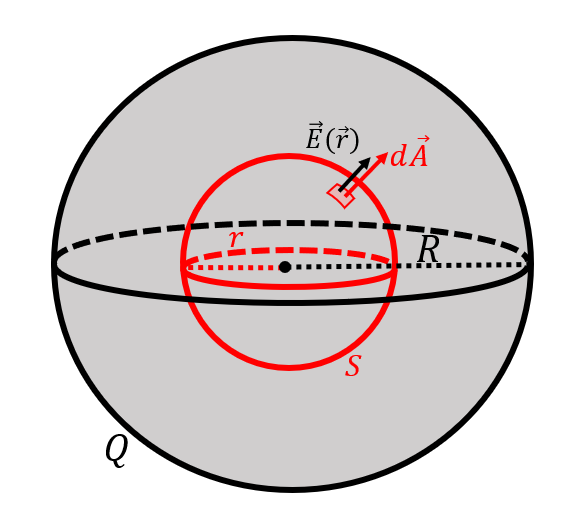
\includegraphics[width=0.4\linewidth]{files/sphereout-6866d16fabe96bb0b0685aa3085b2ab7.png}
\caption[]{A spherical Gaussian surface to determine the electric field inside of a sphere of radius, $R$, holding charge, $+Q$.}
\label{fig:gauss:sphereout}
\end{figure}

The flux integral is trivial again, since the electric field always makes the same angle with the Gaussian surface, and the magnitude of the electric field is constant in magnitude along the surface:
\begin{equation}
\Phi_E&=\oint \vec E\cdot d\vec A=\oint E dA= E\oint dA=E(4\pi r^2)
\end{equation}
In this case, however, the charge in the volume enclosed by the Gaussian surface is less than $Q$, since the whole charge is not enclosed. We are told that the charge is distributed uniformly throughout the spherical volume of radius $R$. We can thus define a volume charge density, $\rho$, (charge per unit volume) for the sphere:
\begin{equation}
\rho=\frac{Q}{V}=\frac{Q}{\frac{4}{3}\pi R^3}
\end{equation}
The volume enclosed by the Gaussian surface is $\frac{4}{3}\pi r^3$, thus the charge, $Q^{enc}$, contained in that volume is given by:
\begin{equation}
Q^{enc}=\frac{4}{3}\pi r^3 \rho=\frac{4}{3}\pi r^3 \frac{Q}{\frac{4}{3}\pi R^3}=Q\frac{r^3}{R^3}
\end{equation}
Finally, we apply Gauss' law to find the magnitude of the electric field inside the sphere:
\begin{equation}
\oint \vec E\cdot d\vec A&=\frac{Q^{enc}}{\epsilon_0} \\
E(4\pi r^2) &=\frac{Q}{\epsilon_0}\frac{r^3}{R^3}\\
\therefore E&= \frac{Q}{4\pi\epsilon_0R^3}r
\end{equation}
Note that the electric field increases linearly with radius inside of the charged sphere, and then decreases with radius squared outside of the sphere. Also, note that at the centre of the sphere, the electric field has a magnitude of zero, as expected from symmetry.

\textbf{Discussion:} In this example, we showed how to use Gauss' law to determine the electric field inside and outside of a uniformly charged sphere. We recognized the spherical symmetry of the charge distribution and chose to use a spherical surface in order to apply Gauss' law.  This, in turn, allowed the flux to be easily calculated. We found that outside the sphere, the electric field decreases in magnitude with radius squared, just as if the entire charge were concentrated at the centre of the sphere. Inside the sphere, we found that the electric field is zero at the centre, and increases linearly with radius.
\end{framed}
\end{framed}

\begin{framed}
\textbf{Olivia's Thoughts}\\
In Section~\ref{chapter:gravity}, I provided an analogy to explain Gauss' law for gravity. If that analogy worked for you, I recommend you revisit it, as the same principles apply here. I'm now going to describe another way to think about Gauss' law that will be useful as you become more familiar with field lines.

Figure~\ref{fig:gauss:sphere_fieldlines} shows the field lines coming from a positively charged sphere, like the one in Example~16.4.

\begin{figure}[!htbp]
\centering
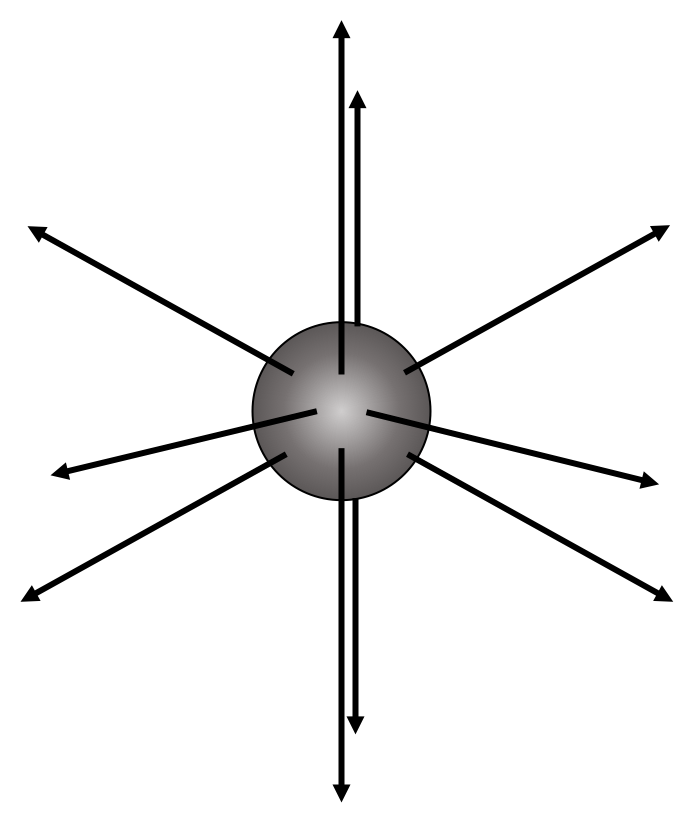
\includegraphics[width=0.3\linewidth]{files/sphere_fieldlines-65b7b440bddcf87b2453dc79de3bf357.png}
\caption[]{The field lines for a positively charged sphere.}
\label{fig:gauss:sphere_fieldlines}
\end{figure}

Let's see what happens when we put a spherical Gaussian surface around the charged sphere. Figure~\ref{fig:gauss:2surfaces_1} shows two surfaces of different sizes.

\begin{figure}[!htbp]
\centering
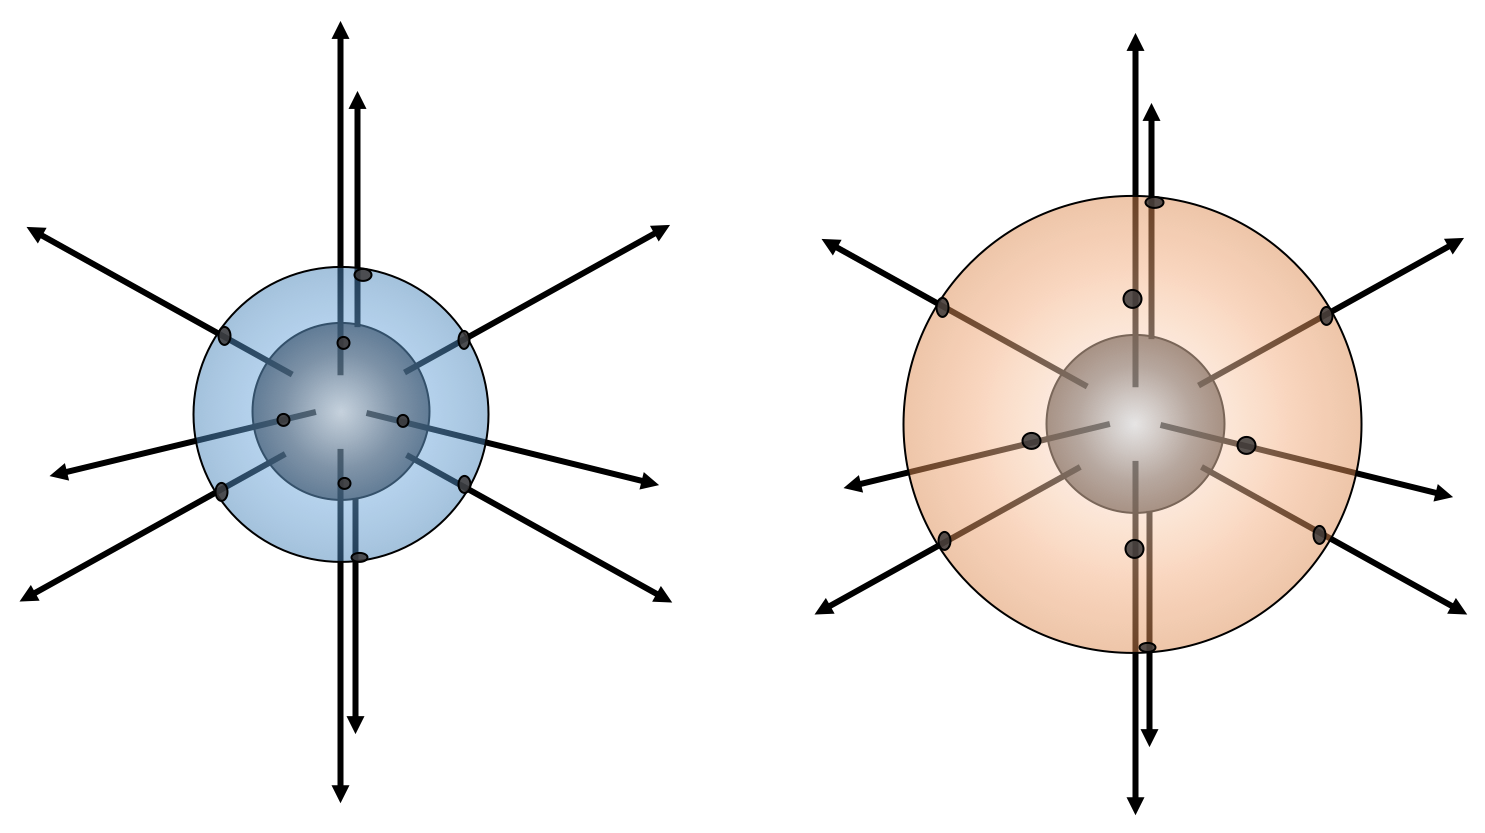
\includegraphics[width=0.6\linewidth]{files/2surfaces_1-d3a5fe6e84b1b1eae3399078f9dfcc82.png}
\caption[]{Two Gaussian surfaces with different radii around a charged sphere.}
\label{fig:gauss:2surfaces_1}
\end{figure}

To make it a bit clearer, I'll now take the charge out of the image (Figure~\ref{fig:gauss:2surfaces_2}), and use dots to show where the field lines passed through each surface.

\begin{figure}[!htbp]
\centering
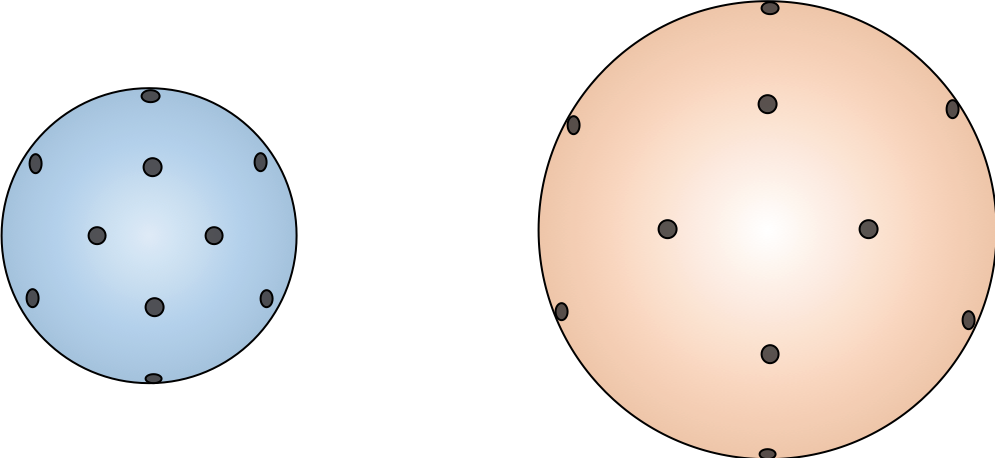
\includegraphics[width=0.5\linewidth]{files/2surfaces_2-7b83365589a0dc3bba79cef83eaf9f3f.png}
\caption[]{The Gaussian surfaces from Figure~\ref{fig:gauss:2surfaces_1}, where the dots show where the field lines passed through each surface.}
\label{fig:gauss:2surfaces_2}
\end{figure}

Gauss' law tells us that, because each surface enclosed the same amount of charge, the same number of field lines will pass through each surface. Therefore, these spheres should have the same number of dots on them. The difference between them is the \textit{density} of the dots. We have learned that the closer the field lines are to each other, the stronger the electric field is. So, if we wanted to know the magnitude of the electric field at some point on one of these surfaces, we would calculate the number field lines passing through it, and then divide by the area of the sphere to get the density of the field lines.

Let's revisit the equation for Gauss' law,
\begin{equation}
\oint \vec E\cdot d\vec A=\frac{Q^{enc}}{\epsilon_0}
\end{equation}
The right hand side gives us the number of field lines (the flux). If we can construct a surface so that the field lines passing through it are evenly distributed (and they are perpendicular to the surface), the left hand side becomes $\oint \vec E\cdot d\vec A= EA$. To solve for the electric field, we write $E=Q^{enc}/(\epsilon_0A)$, which is effectively saying that the electric field is equal to the number of field lines divided by the area of the surface.
\end{framed}

\begin{framed}
\textbf{Checkpoint}\\
\begin{figure}[!htbp]
\centering
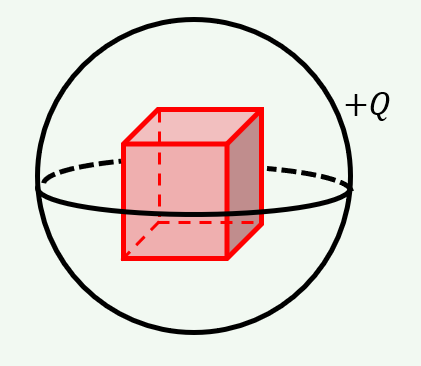
\includegraphics[width=0.3\linewidth]{files/spherecube-975b218a76380121f84eee937fcc1c53.png}
\caption[]{A charged spherical shell with a cubic device inside of it.}
\label{fig:gauss:spherecube}
\end{figure}

A thin charged spherical shell carries a uniformly distributed charge of $+Q$. If we place a cube inside the shell, as shown in Figure~\ref{fig:gauss:spherecube}, what is the total flux out of the surface of the cube?

\begin{enumerate}
\item $\frac{Q}{12\pi}{\rm Vm}$.
\item $\frac{Q}{2\pi} {\rm Vm}$.
\item $\frac{Q}{6} {\rm Vm}$.
\item $0 {\rm Vm}$.
\end{enumerate}

\begin{framed}
\textbf{Answer}\\
\begin{enumerate}[resume]
\item
\end{enumerate}
\end{framed}
\end{framed}

\begin{framed}
\textbf{Example 16.5}\\
An infinitely long straight wire carries a uniform charge per unit length, $\lambda$. What is the electric field at a distance, $R$, from the wire?\}
The first thing we want to do is determine the direction of the electric field vector. We start by making a diagram of the charge distribution, as in Figure~\ref{fig:gauss:linecharge}. To choose the direction, we can use symmetry arguments. In this case,  our choice of field direction must preserve rotational symmetry. This means that if we are in the plane perpendicular to the wire (i.e. the side view in Figure~\ref{fig:gauss:linecharge}), the electric field should look the same from all directions (e.g. it shouldn't matter if we look at it from the left side or the right side). With this in mind, there are three options for the electric field. It could be either:

\begin{enumerate}
\item in the radial direction (point to/from the centre of the wire).
\item such that electric field lines form concentric circles with the wire.
\item co-linear with the wire.
\end{enumerate}

\begin{framed}
\textbf{Solution}\\
In all three possibilities above, you would not be able to infer that one particular direction in the plane perpendicular to the wire is preferred. All three possibilities preserve the rotational symmetry of the wire (the wire looks the same from all directions in the plane perpendicular to the wire).

We expect that a a negative charge would be attracted to the wire, so the electric field should have at least some radial component. We can thus eliminate the second and third options. The electric field will must then look like that illustrated in Figure~\ref{fig:gauss:linecharge}.

\begin{figure}[!htbp]
\centering
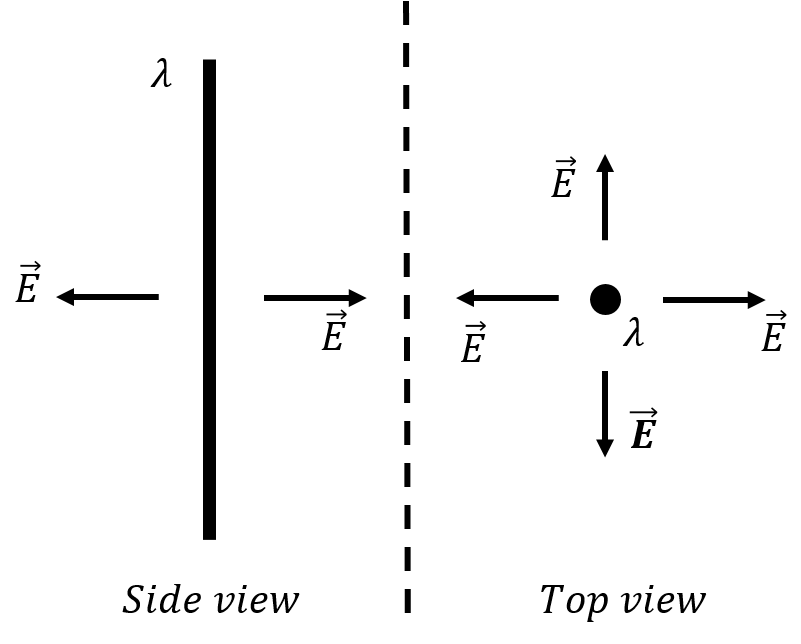
\includegraphics[width=0.4\linewidth]{files/linecharge-4014db5a513bae16bff2ff03bbbcfb09.png}
\caption[]{An infinite line of charge carrying uniform charge per unit length, $\lambda$. The left panel shows a side view and the right panel a view from above. The electric field must be in the radial direction or there would be a preferred direction.}
\label{fig:gauss:linecharge}
\end{figure}

Next, we need to choose a Gaussian surface in order to apply Gauss' law. A convenient choice is a cylinder (a ``pill box'') of radius $R$ and length $L$, as shown in Figure~\ref{fig:gauss:fluxlinecharge}, as this goes through a point that is a distance $R$ from the wire (where we are asked for the electric field). At all points on the cylindrical surface, the electric field vector is either perpendicular or parallel to the surface.

\begin{figure}[!htbp]
\centering
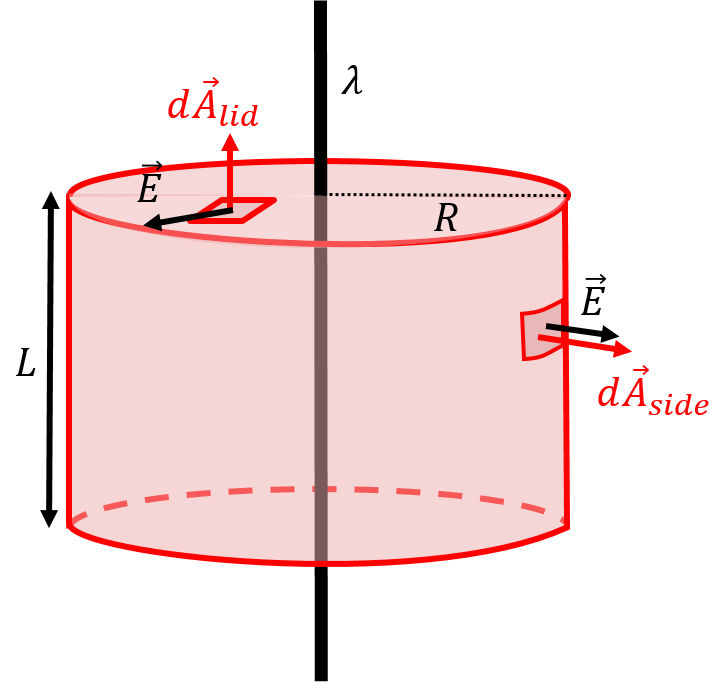
\includegraphics[width=0.4\linewidth]{files/fluxlinecharge-5050ac892660d0dcaa40a8b7c9eb94a3.png}
\caption[]{A cylindrical Gaussian surface is used to calculate the flux from an infinite line of charge.}
\label{fig:gauss:fluxlinecharge}
\end{figure}

We can think of the cylindrical surface as being composed of three surfaces: two disks on either end (the lids of the pill box), and the curved surface that makes up the side of the cylinder. The flux through the entire cylindrical surface will be the sum of the fluxes through the two lids plus the flux through the side:
\begin{equation}
\oint \vec E\cdot d\vec A = \int_{side} \vec E\cdot d\vec A + \int_{lid}\vec E\cdot d\vec A + \int_{lid}\vec E\cdot d\vec A
\end{equation}
where you should note that the closed integral ($\oint$) was separated into three normal integrals ($\int$) corresponding to the three ``open'' surfaces that make up the closed surface. Again, remember that the flux is proportional to the net number of field lines exiting/entering the closed surface, so it makes sense to count those lines over the three open surfaces and add them together to get the total number for the closed surface.

The flux through the lids is identically zero, since the electric field is perpendicular to $d\vec A$ everywhere on the lids. The total flux is therefore equal to the flux through the curved side surface, for which the electric field vector is always parallel to $d\vec A$, and for which the electric field vector is constant in magnitude:
\begin{equation}
\oint \vec E\cdot d\vec A = \int_{side} \vec E\cdot d\vec A =\int_{side} EdA=E\int_{side}dA=E(2\pi R L)
\end{equation}
where we recognized that the side surface can be unfolded into a rectangle of height $L$ and width $2\pi R$, corresponding to the circumference of the cylinder, so that the area of the side of the cylinder is given by $A=2\pi R L$.

Next, we determine the charge inside the volume enclosed by the surface. Since the cylinder encloses a length $L$ of wire, the enclosed charge is given by:
\begin{equation}
Q^{enc}=\lambda L
\end{equation}
where $\lambda$ is the charge per unit length on the wire. Putting this all together into Gauss' law gives us the electric field at a distance $R$ from the wire:
\begin{equation}
\oint \vec E\cdot d\vec A&=\frac{Q^{enc}}{\epsilon_0} \\
E(2\pi R L) &= \frac{\lambda L}{\epsilon_0}\\
\therefore E&= \frac{\lambda}{2\pi\epsilon_0R}
\end{equation}
Note that this is the same result that we obtained in Example~15.5, when we took the limit of the finite line of charge having infinite length.

\textbf{Discussion:} In this example, we applied Gauss' law to determine the electric field at a distance from an infinitely long charged wire. We used symmetry to argue that the field should be radial and in the plane perpendicular to the wire, and recognized that a cylindrical Gaussian surface would exploit the symmetry so that the flux can easily be calculated. We obtained the same result as we did from integrating Coulomb's Law in Example~15.5. However, using Gauss' law was much less work than integrating Coulomb's Law.
\end{framed}
\end{framed}

\begin{framed}
\textbf{Checkpoint}\\
Why is it difficult to apply Gauss' law to a finite wire?

\begin{enumerate}
\item It is easy to apply Gauss' law to a finite wire.
\item Because the flux of a finite wire is undefined.
\item Because we do not know the charge density of a finite wire.
\item Because the symmetry argument does not hold.
\end{enumerate}

\begin{framed}
\textbf{Answer}\\
\begin{enumerate}[resume]
\item
\end{enumerate}
\end{framed}
\end{framed}

\begin{framed}
\textbf{Josh's Thoughts}\\
Gauss' law requires us to choose a ``Gaussian'' surface, but which surface should we choose? Generally, it is useful to choose a surface such that the flux can easily be determined, ideally without having to actually do an integral. If symmetry can be exploited such that $\vec E$ has a constant magnitude and direction relative to $d\vec A$ at every location of the Gaussian surface, then $\int \vec E \cdot d\vec A$ will be equal to $E A$. This is why Gaussian surfaces are often of the same shape as the charged object they are enclosing.

For example, if I need to enclose a cylindrical charge, it would be reasonable to enclose the charge with a cylindrical Gaussian surface, as shown in Figure~\ref{fig:gauss:choosecylinder}

\begin{figure}[!htbp]
\centering
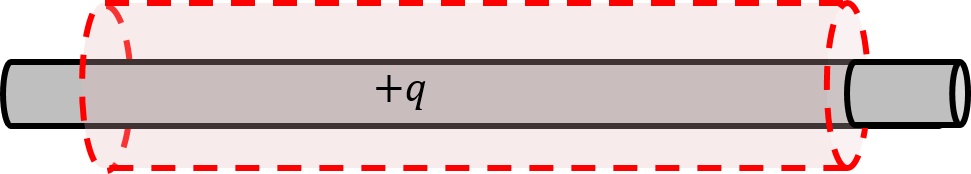
\includegraphics[width=0.3\linewidth]{files/choosecylinder-eda869a34c5238cae536651ec6a93e68.png}
\caption[]{A cylindrical Gaussian surface to enclose a cylindrical charge.}
\label{fig:gauss:choosecylinder}
\end{figure}

When dealing with point charges which have no shape and are thus spherically symmetric, it makes sense to choose a spherical Gaussian surface, as shown in Figure~\ref{fig:gauss:choosesphere}, since the electric field is in the radial direction for a point charge.

\begin{figure}[!htbp]
\centering
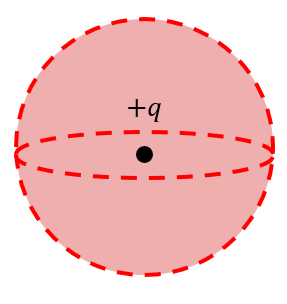
\includegraphics[width=0.2\linewidth]{files/choosesphere-bfbaa81e8b4c4b6ad75bf006d36063dd.png}
\caption[]{. A spherical Gaussian surface to enclose a point charge.}
\label{fig:gauss:choosesphere}
\end{figure}

Finally, there are some cases of less than ideal choices for the Gaussian surfaces. While never wrong, they may require rather complicated integrals to determine the flux. These cases will still provide a correct answer if the situation is modelled correctly.

Suppose that I enclose a spherical charge with a cylindrical Gaussian surface, as shown in Figure~\ref{fig:gauss:dontchoosecylinder}. The electric field will be stronger near the middle of the cylinder's length than at the centre of its end caps, which means that $\vec E$ is not constant in $\int \vec E \cdot d \vec A$, so the integral cannot be simplified to $EA$. A better choice for a Gaussian surface in this case would be a sphere, which exploits the symmetry of the charge distribution and results in a $\vec E$ of constant magnitude everywhere along the surface. Figure~\ref{fig:gauss:fluxdA} and Figure~\ref{fig:gauss:fluxlinx} give other examples of when we cannot assume $\Phi$ to be equal to $EA$.

\begin{figure}[!htbp]
\centering
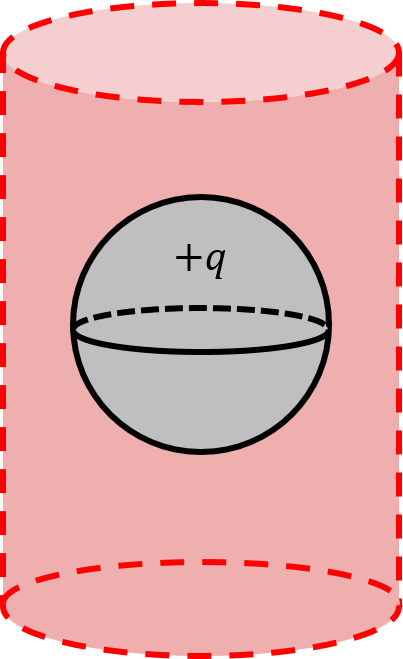
\includegraphics[width=0.2\linewidth]{files/dontchoosecylinder-ab9276b288b9db308f37157107ffbc73.png}
\caption[]{. A cylindrical surface is not a good choice to enclose a spherical charge.}
\label{fig:gauss:dontchoosecylinder}
\end{figure}
\end{framed}

\begin{framed}
\textbf{Example 16.6}\\
Determine the electric field above an infinitely large plane of charge with uniform surface charge per unit area, $\sigma$.

\begin{framed}
\textbf{Solution}\\
Figure~\ref{fig:gauss:plane} shows a portion of the infinite plane. The electric field vector must be perpendicular to the plane or a preferred direction could otherwise be inferred from the direction of the electric field. We can also argue that the horizontal components of the electric field will cancel everywhere above the plane, since the plane is infinite. The electric field will point away from the plane if the charge is positive, and towards the plane if the charge is negative.

\begin{figure}[!htbp]
\centering
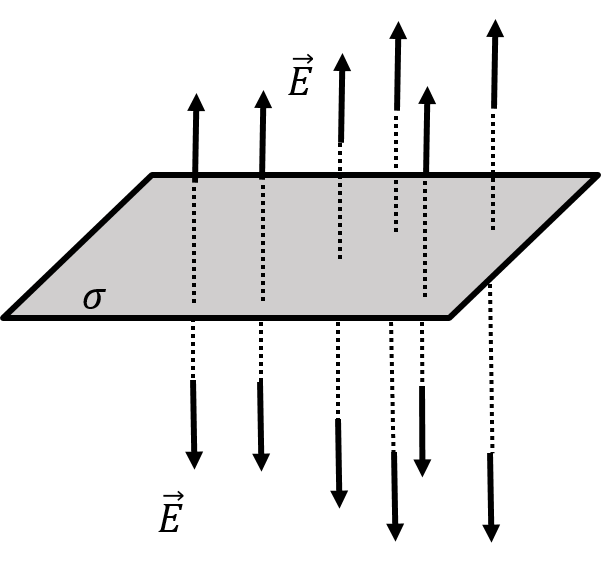
\includegraphics[width=0.4\linewidth]{files/plane-d0a96e90ca3e3d639d338b307ecccab8.png}
\caption[]{The electric field above an infinite plane with uniform charge per unit area, $\sigma$, must be perpendicular to the plane.}
\label{fig:gauss:plane}
\end{figure}

A cylindrical or box-shaped Gaussian surface would both lead to the flux integral being easy to calculate, as illustrated in Figure~\ref{fig:gauss:fluxplane}. Indeed, since the electric field is perpendicular to the plane, only the parts of the surface that are parallel to the plane (the lids on the cylinder, the two horizontal planes in the box) will have a net flux through them.

\begin{figure}[!htbp]
\centering
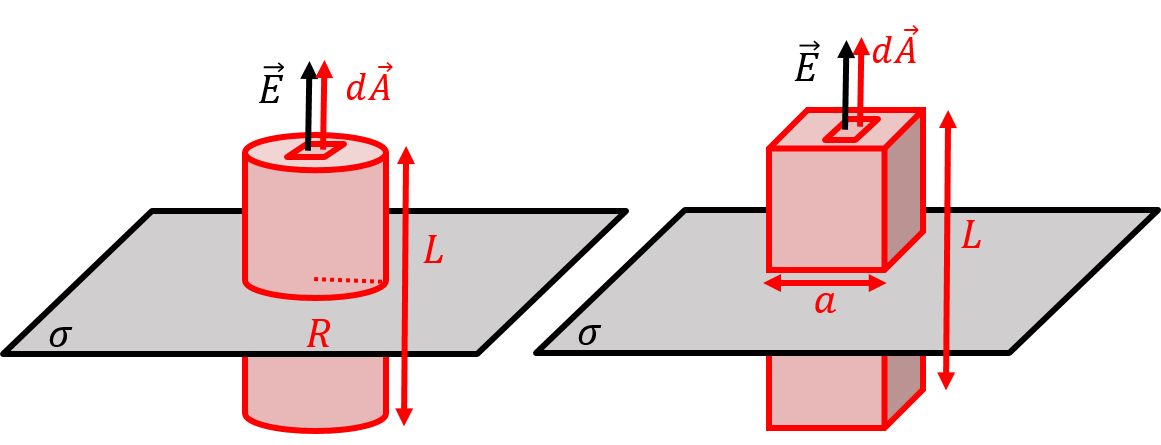
\includegraphics[width=0.8\linewidth]{files/fluxplane-699ae1b062d45554f05fd11d04c847bd.png}
\caption[]{A cylindrical surface or a box are both good choices for a Gaussian surface above a plane, since only the parts of the surface parallel to the plane will have net flux through them.}
\label{fig:gauss:fluxplane}
\end{figure}

Let us choose a box (right panel of Figure~\ref{fig:gauss:fluxplane}) of length, $L$, with a square cross-section of side, $a$. We place the box such that the plane intersects the centre of the box (although this is not required, since we already know that the electric field will not depend on distance from the plane). The flux through the box is simply the flux through the two horizontal planes (of area $a^2$):
\begin{equation}
\oint \vec E\cdot d\vec A&= \int_{top} EdA+\int_{bottom}EdA=2Ea^2
\end{equation}
The box encloses a section of the plane with area $a^2$, so that the net charge enclosed by the surface is:
\begin{equation}
Q^{enc}=\sigma a^2
\end{equation}
Applying Gauss' law allows us to determine the magnitude of the electric field:
\begin{equation}
\oint \vec E\cdot d\vec A&=\frac{Q^{enc}}{\epsilon_0} \\
2Ea^2&= \frac{\sigma a^2}{\epsilon_0}\\
\therefore E&= \frac{\sigma}{2\epsilon_0}
\end{equation}
which is the same result that we found in Example~15.6.

\textbf{Discussion:} In this example, we used Gauss' law to determine the electric field above an infinite plane. We found that we had a choice of Gaussian surfaces (cylinder, box) that allowed us to apply Gauss' law. We found the same result that we had found in Example~15.6 where we had integrated Coulomb's Law (twice, once for a ring of charge, then for a disk, then took the limit of the disk radius going to infinity). Again, we see that in configurations with a high degree symmetry, Gauss' law can be very straightforward to apply.
\end{framed}
\end{framed}

\subsubsection{Charges in a conductor}\label{sec:gauss:conductors}

We can use Gauss' law to understand how charges arrange themselves on a conductor. Consider an infinite plane that carries a total charge per unit area, $\sigma$, similar to what we considered in Example~16.6. In this case, we explicitly consider the plane to be a conductor and to have a finite thickness. If we zoom into the plane, we can illustrate that the charges are located on the surface of the plane, as illustrated in Figure~\ref{fig:gauss:fluxconductingplane}, where the plane is seen edge on. Thus, the \textbf{charge density at the surface is half of the total charge density} of the plane.

\begin{figure}[!htbp]
\centering
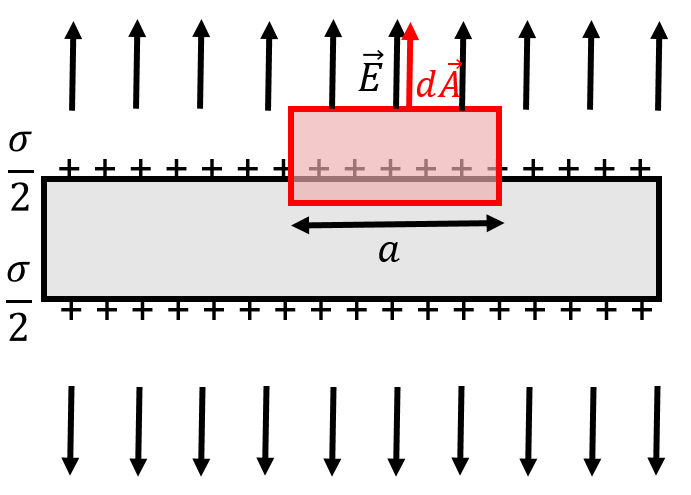
\includegraphics[width=0.4\linewidth]{files/fluxconductingplane-1c0be40aaf0892d7a87ea45a940a18c3.png}
\caption[]{Cross-section of a conducting plane where the charges migrate to the surface. A box-shaped Gaussian surface is also shown as seen from the side (the third dimension of the box is perpendicular to the plane of the page).}
\label{fig:gauss:fluxconductingplane}
\end{figure}

To determine the electric field near the plane, we choose a Gaussian surface that is a box (as in Example~16.6), but require the lower end of the box to go through the plane, as illustrated in Example~16.6. With this choice of Gaussian surface, only the top surface (area $a^2$) will have flux through it, since the \textbf{electric field inside a conductor must be zero}\footnote{Since charges can freely move in a conductor, they will move until there is no reason to move. Eventually, the charges accumulate in such a way that the net field in the conductor is zero. For a plane, this means that half of the charges will move to each side, as illustrated.}. The total flux is given by:
\begin{equation}
\oint \vec E\cdot d\vec A&= \int_{top} EdA=Ea^2
\end{equation}
The charge enclosed is given by:
\begin{equation}
Q^{enc}=\frac{\sigma}{2}a^2
\end{equation}
where we used the fact that only half of the charges are inside the volume enclosed by our Gaussian surface, so that the charge per unit area is half ($\frac{\sigma}{2}$) of that for the entire plane. Applying Gauss' law, we find that the electric field is given by:
\begin{equation}
\oint \vec E\cdot d\vec A&=\frac{Q^{enc}}{\epsilon_0} \\
Ea^2&= \frac{\sigma a^2}{2\epsilon_0}\\
\therefore E&= \frac{\sigma}{2\epsilon_0}\quad \text{(Field above an infinite plane)}
\end{equation}
as in Example~16.6, but now the factor of two comes from having half of the charge density, whereas before it was because two of the faces of the box had non-zero flux. We can generalize this result to determine the electric field near the surface of any conductor. Very close to the surface of any object, one can consider the surface as being similar to an infinite plane. If that surface carries charge per unit area, $\sigma$, then the electric field just above the surface is given by:
\begin{equation}
E&= \frac{\sigma}{\epsilon_0} \quad \text{(Field near a conducting surface)}
\end{equation}
In this case, there is no factor of two because the charge density in this equation is the charge density of the conductor (not the charge density one side of the surface). In the previous equation, the charge density on the surface of the conducing plane was $\frac{\sigma}{2}$.

Consider, now, a neutral spherical conducting shell, as shown from the side in the left panel of Figure~\ref{fig:gauss:sphereshell}. When a charge, $+Q$, is placed at the centre of the shell (right panel), charges inside the shell will move until the field inside the conducting material of the shell is identically zero. The negative charges will move towards the inner surface (as they are attracted to $+Q$) and positive charges will be repelled onto the outer surface, under the influence of the electric field created by $+Q$ (shown in the diagram as $\vec E_{Q}$). Eventually, the separation of charges will lead to an electric field (shown in the diagram as $\vec E_{\sigma}$) in the opposite direction. The charges will stop moving once the total electric field in the conductor is zero (when the two fields cancel exactly everywhere in the conductor).

\begin{figure}[!htbp]
\centering
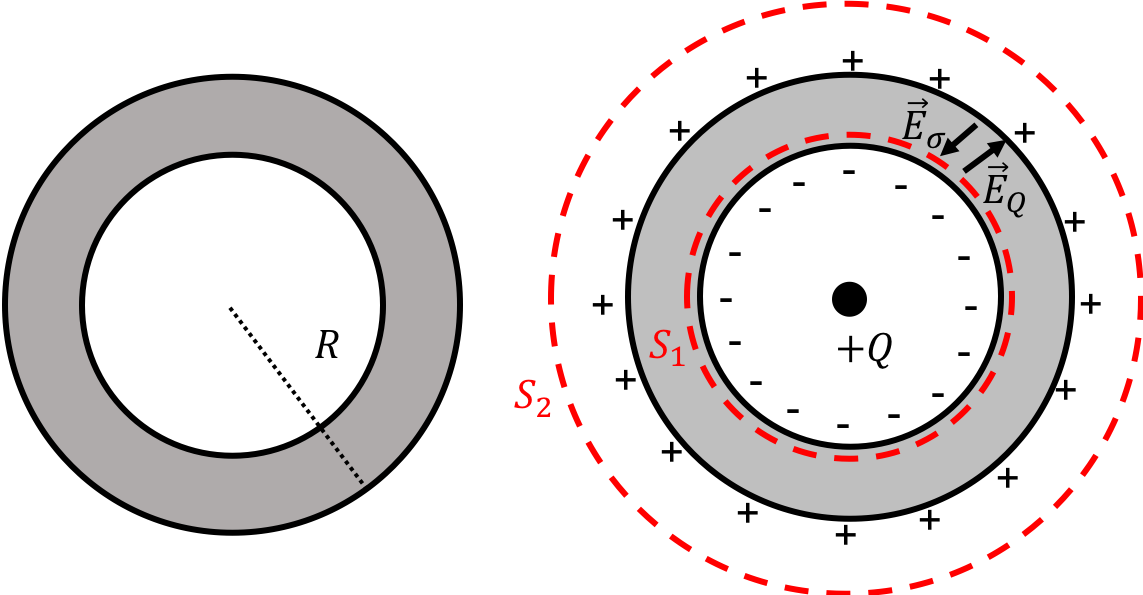
\includegraphics[width=0.7\linewidth]{files/sphereshell-9b7f9182300681b8ecbe7b3c10387400.png}
\caption[]{Left: a neutral conducting spherical shell (seen edge on). Right: A positive charge, $+Q$, placed at the centre of the shell. Charges in the shell will separate in order to keep the electric field inside the conductor zero.}
\label{fig:gauss:sphereshell}
\end{figure}

We can use Gauss' law to determine the amount of charge that has accumulated on the inner surface. Consider the Gaussian spherical surface, $S_1$, in Figure~\ref{fig:gauss:sphereshell}, that is concentric with the shell and has a radius such that the surface is just inside the shell. Since the electric field is zero inside the shell, the flux out of the Gaussian surface must be zero. By Gauss' law, the amount of charge enclosed by the surface must also be zero. Thus, a total charge, $-Q$, will have accumulated on the inner surface of the conductor (since $Q^{enc}= -Q+Q=0$). Because one cannot just create charge from nothing, there must be an equal amount of opposite charge, $+Q$, on the outer surface of the shell. This is true of any conducting material with a cavity inside of it: if you place a charge $+Q$ in the cavity, a charge $-Q$ will accumulated on the inner surface and a charge $+Q$ will accumulate on the outer surface.

Now consider the flux out of the surface $S_2$, which is outside of the shell. The net charge enclosed will be $Q^{enc}=+Q -Q+Q=+Q$. If we say that the radius of $S_2$ is $r$,  then the flux out of the spherical surface is given by:
\begin{equation}
\oint \vec E\cdot d\vec A &= E(4\pi r^2)\\
\end{equation}
and the electric field, from Gauss' law, is simply that of a point charge, $+Q$:
\begin{equation}
E&=\frac{1}{4\pi\epsilon_0}\frac{Q}{r^2}
\end{equation}
and the shell has no effect on the field. Right at the surface of the shell (outer radius $R$), the surface charge density is given by:
\begin{equation}
\sigma=\frac{Q}{4\pi r^2}
\end{equation}
Above, we found the electric field at the surface of a conductor that carries charge per unit area, $\sigma$, to be:
\begin{equation}
E&= \frac{\sigma}{\epsilon_0}
\end{equation}
which is clearly the same result that we obtained using the spherical surface, $S_2$:
\begin{equation}
E&= \frac{\sigma}{\epsilon_0}=\frac{1}{4\pi\epsilon_0}\frac{Q}{r^2}
\end{equation}
Note that we found the electric field using Gauss' law only in this last case, and found it to be equal to the electric field that one obtains from Coulomb's law. Thus, Gauss' law only works if the field has an ``inverse square law'' dependence. If Gauss' law does not provide the correct electric field, then the force does not depend on $1/r^2$. Gauss' law can be used to make extremely stringent tests of whether the force goes as $1/r^2$ or deviates from this model.

\subsubsection{Interpretation of Gauss' law and vector calculus}\label{sec:gauss:interpretation}

In this section, we provide a little more theoretical background and intuition on Gauss' law, as well as its connection to vector calculus (which is beyond the scope of this textbook, but interesting to have a feeling for). Very generally, Gauss' law is a statement that connects a property of a vector field to the ``source'' of that field. We think of mass as the source for the gravitational field, and we think of charge as the source for the electric field. The property of the field that we considered in this case was its ``flux out of a closed surface''.

Recall that determining the flux of a field out of a closed surface is equivalent to counting the net number of field lines that exit that closed surface. Field lines must start on a positive charge and must end on a negative charge. Thus, if there is a net number of field lines exiting the surface, there must be a positive charge in the volume defined by the surface (a ``source'' of field lines). If there is a net number of field lines entering the surface, then the volume defined by the surface must enclose a negative charge (a ``sink'' of field lines). Gauss' law is simply a statement that the number of field lines entering/exiting a closed surface is proportional to the amount of charge enclosed in that volume.

The flux out of a closed surface is tightly connected to the vector calculus concept of ``divergence'', which describes whether field lines are diverging (spreading out or getting closer together). When a point charge is present, field lines will emanate radially from that point charge; in other words, they will diverge. We say that the electric field has non-zero divergence if there is a source of the electric field in that position of space. The key difference between the concept of divergence and that of ``flux out of a closed surface'', is that divergence is a local property of the field (it is true at a point), whereas the flux out of a surface must be calculated using a finite volume and makes it challenging to define the field at a specific position. Gauss' law defined using flux is thus not as useful for describing how the field changes at specific positions, and is usually limited to situations with a high degree of symmetry.

The divergence, $\nabla \cdot \vec E$, of a vector field, $\vec E$, at some position is defined as:
\begin{equation}
\nabla \cdot \vec E=\frac{\partial E}{\partial x}+\frac{\partial E}{\partial y}+\frac{\partial E}{\partial z}
\end{equation}
and corresponds to the sum of three partial derivatives evaluated at that position in space. Gauss' theorem (also called the divergence theorem) states that:
\begin{equation}
\int_V \nabla \cdot \vec E = \oint_S \vec E \cdot d\vec A
\end{equation}
where the subscript on the integral indicates whether the sum (integral) should be carried out over a volume, $V$, or over a closed surface, $S$, as we have practised in this chapter. While it is not important at this level to understand the theorem in detail, the point is that one can convert a ``flux over a closed surface'' into an integral of the divergence of the field. In other words, we can convert a global property (flux) to a local property (divergence). Gauss' law in terms of divergence can be written as:
\begin{equation}
\boxed{\nabla \cdot \vec E = \frac{\rho}{\epsilon_0}}\quad \text{(Local version of Gauss' law)}
\end{equation}
where $\rho$ is the charge per unit volume at a specific position in space. This is the version of Gauss' law that is usually seen in advanced textbooks and in Maxwell's unified theory of electromagnetism. This version of Gauss' law relates a local property of the field (its divergence) to a local property of charge at that position in space (the charge per unit volume at that position in space). If we integrate both sides of the equation over volume, we recover the original formulation of Gauss' law: the left hand side, by the divergence theorem, leads to flux when integrated over volume, whereas on the right hand side, the integral over volume of charge per unit volume, $\rho$, will give the total charge enclosed in that volume, $Q^{enc}$:
\begin{equation}
\int_V  \left(\nabla \cdot \vec E \right)dV&= \int_V \left(\frac{\rho}{\epsilon_0}\right) dV\\
\oint_S \vec E \cdot d\vec A &=\frac{Q^{enc}}{\epsilon_0}
\end{equation}

\subsubsection{Summary}

We can define the \textbf{flux} of a uniform and constant vector field, $\vec E$, through a flat surface, as:
\begin{equation}
\Phi_E = \vec E \cdot \vec A = EA\cos\theta
\end{equation}
where $\vec A$ is a vector that is perpendicular to the surface with a magnitude equal to the area of that surface, and, $\theta$, is the angle between $\vec A$ and $\vec E$.

The flux of a field through a surface is proportional to the number of field lines that cross that surface. If the surface is parallel to the field ($\vec A$ and $\vec E$ are thus perpendicular), the flux through that surface is zero (no field lines cross the surface, the scalar product is zero). If $\vec E$ and $\vec A$ change over the surface ($\vec E$ and/or $\vec A$ change magnitude and/or direction relative to each other along the surface), then we treat the surface as being made of infinitesimal surface elements over which the two vectors are constant. We define a vector $d\vec A$ to be perpendicular to the surface element with an infinitesimal area, $dA$. The total flux is then obtained by summing the fluxes through each surface element:
\begin{equation}
\Phi_E=\int \vec E \cdot d\vec A=\int EdA\cos\theta
\end{equation}
Note that the direction of the vector $d\vec A$ (or $\vec A$) is ambiguous, as one can choose either of two directions perpendicular to a surface. Usually, one chooses the direction of $\vec A$ so that the flux is positive (i.e. $\vec A$ has a component parallel to $\vec E$). However, if the surface is ``closed'' (that is, it defines a volume), then we always choose the direction of $d\vec A$ so that it points outwards from the surface (since the surface encloses a volume, one can define an ``inside'' and an ``outside'').

In the case of the electric field, Gauss' law relates the flux of the electric field from a closed surface to the amount of charge, $Q^{enc}$, contained in the volume enclosed by that surface:
\begin{equation}
\oint \vec E \cdot d\vec A = \frac{Q^{enc}}{\epsilon_0}
\end{equation}
Physically, Gauss' law is a statement that field lines must begin or end on a charge (electric field lines originate on positive charges and terminate on negative charges). If there is a net number of lines coming out of a closed surface (a positive flux), that surface must enclose a positive charge from where those field lines originate. Similarly, if there are the same number of field lines entering a closed surface as there are lines exiting that surface (a flux of zero), then the surface encloses no charge. Gauss' law states that the number of field lines exiting a closed surface is proportional to the amount of charge enclosed by that surface.

Gauss' law is useful to determine the electric field. However, this can only be done analytically for charge distributions with a very high degree of symmetry. This is because the flux integral is not usually easy to evaluate unless:

\begin{enumerate}
\item \textbf{The electric field makes a constant angle with the surface}. When this is the case, the scalar product can be written in terms of the cosine of the angle between $\vec E$ and $d\vec A$, which can be taken out of the integral if it is constant:
\end{enumerate}
\begin{equation}
\oint \vec E\cdot d\vec A=\oint E\cos\theta dA=\cos\theta\oint EdA
\end{equation}
\begin{enumerate}[resume]
\item \textbf{The electric field is constant in magnitude along the surface}. When this is the case, the integral can be simplified further by factor out $E$, and simply becomes an integral over $dA$ (which corresponds to the total area of the surface, $A$):
\end{enumerate}
\begin{equation}
\oint \vec E\cdot d\vec A=\cos\theta\oint EdA =E\cos\theta\oint dA=EA\cos\theta
\end{equation}
Note that Gauss' law does not specify a closed surface over which to calculate the flux; it holds for any surface. We can thus choose a surface that will make the flux integral easy to evaluate - we call this choice a ``Gaussian surface'' (not because it has some special property, but because we chose that surface to apply Gauss' law). A procedure for applying Gauss' law to determine the electric field at some point in space can be written as:

\begin{enumerate}
\item Make a diagram showing the charge distribution.
\item Use symmetry arguments to determine in which way the electric field vector points.
\item Choose a Gaussian surface that goes through the point for which you want to know the electric field. Ideally, the surface is such that the electric field is constant in magnitude and always makes the same angle with the surface, so that the flux integral is straightforward to evaluate.
\item Calculate the flux, $\oint \vec E\cdot d\vec A$.
\item Calculate the amount of charge in the volume enclosed by the surface, $Q^{enc}$.
\item Apply Gauss' law, $\oint \vec E\cdot d\vec A=\frac{Q^{enc}}{\epsilon_0}$.
\end{enumerate}

We showed how Gauss' law can be used to understand and quantify how charges arrange themselves on a conductor, in such a way that the electric field is zero everywhere in the conductor. Finally, we briefly introduced a more modern version of Gauss' law that uses divergence instead of flux:
\begin{equation}
\nabla \cdot \vec E &= \frac{\rho}{\epsilon_0}
\end{equation}
This last version has the advantage that it relates a local property of the field (divergence) to a local property of charge (charge density at some position in space).

\begin{framed}
\textbf{Important Equations}\\
\textbf{Gauss' Law:}
\begin{equation}
\Phi & = \frac{Q_{enc}}{\epsilon_0}\\
\Phi &= \int \vec E \cdot d \vec A
\end{equation}
\end{framed}

\begin{framed}
\textbf{Important Definitions}\\
\begin{itemize}
\item \textbf{Electric flux:} A measure of the number of electric field lines crossing a surface. SI units: ${\rm \left[{Vm}\right]}$. Common variable(s): $\Phi_E$.
\end{itemize}
\end{framed}

\subsubsection{Thinking about the material}

\begin{framed}
\textbf{Reflect and research}\\
\begin{itemize}
\item Could Gauss' law be applied to magnetism? Why or why not?
\item What else has Gauss done?
\item Are there other interaction for which Gauss' law can be applied?
\item What are Maxwell's equations?
\item How are measurements of flux used in environmental research?
\item How does one use Gauss' law to test the $1/r^2$ dependence of Coulomb's Law?
\end{itemize}
\end{framed}

\begin{framed}
\textbf{To try in the lab}\\
\begin{itemize}
\item Propose an experiment to measure the charge of an object using Gauss' law.
\item Propose an experiment to measure the electric field of a charged object, then compare your experimental results to the theoretical results predicted calculated by Gauss' law.
\item Simulate the surface charge distribution on the inside and outside of a conducting cubic shell which encloses a point charge.
\end{itemize}
\end{framed}

\subsubsection{Sample problems and solutions}

\paragraph{Problems}

\begin{framed}
\textbf{Problem 16.1}\\
Consider a charged sphere of radius $R$, which has a non-uniform charge density that varies as $\rho(r) = ar^2$.

\begin{itemize}
\item a.  What is the total charge of the sphere?
\item b. What is the electric field as a function of distance from the centre of the sphere outside the sphere, $r>R$?
\item c. What is the electric field as a function of distance from the centre of the sphere inside the sphere, $r\leq R$?
\end{itemize}
\end{framed}

\begin{framed}
\textbf{Problem 16.2}\\
A long insulating wire with charge per unit length $+\lambda$ is surrounded by a coaxial conducting shell with charge per unit length $-2\lambda$. You can assume that both the wire and the shell are infinitely long. The inner surface of the shell has a circular cross section of radius $R$. The cross section of the outer surface is an equilateral triangle with side length $L$.

\begin{itemize}
\item a. What is the average surface charge density, $\sigma_{in}$, on the inner surface of the conducting shell?
\item b. What is the average surface charge density, $\sigma_{out}$, on the outer surface of the conducting shell?
\end{itemize}

\begin{figure}[!htbp]
\centering
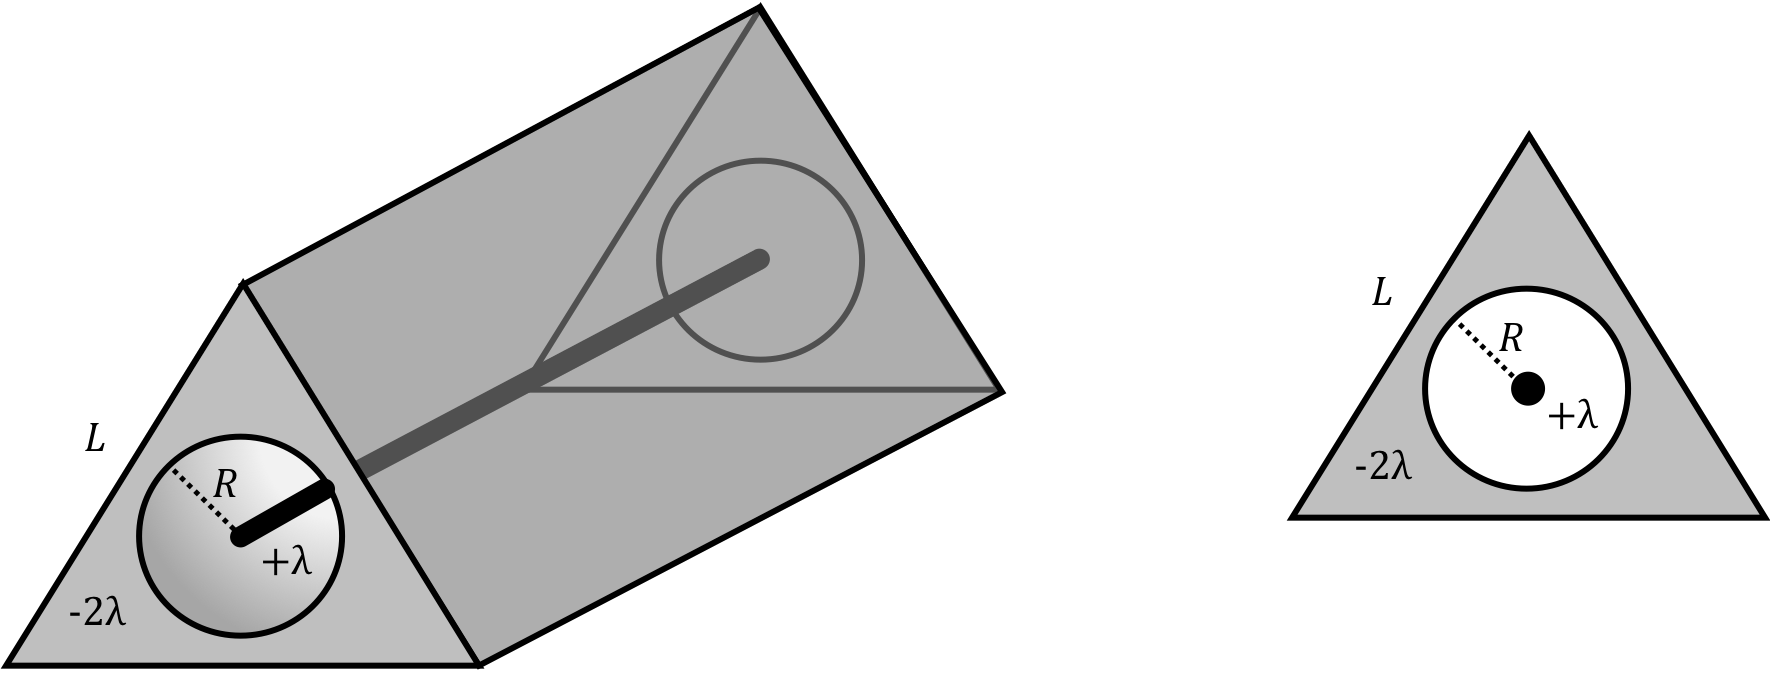
\includegraphics[width=0.8\linewidth]{files/coaxial_triangle-ae2491e601ad23ad3a7ca4bfe406a2d7.png}
\caption[]{Left: Wire surrounded by a conducting shell with a cylindrical inner surface and triangular outer surface. Right: Cross section of the set-up.}
\label{fig:gauss:coaxial_triangle}
\end{figure}
\end{framed}

\paragraph{Solutions}

\begin{framed}
\textbf{Solution 16.1}\\
\begin{itemize}
\item a. In order to determine the total charge of the sphere, we divide the sphere into shells of radius $r$ and infinitesimal thickness $dr$. The volume, $dV$, of a shell is given by its surface area multiplied by its thickness:
\end{itemize}
\begin{equation}
dV = 4\pi r^2 dr
\end{equation}
We can obtain the charge, $dQ$, of each shell by using the charge per unit volume, $\rho(r)$:
\begin{equation}
dQ = \rho(r) dV = ar^24\pi r^2 dr = 4a\pi r^4 dr
\end{equation}
The total charge of the sphere is found by summing the charges from each shell over the radius of the sphere:
\begin{equation}
Q=\int dQ =\int_0^R4a\pi r^4 dr=\frac{4}{5}a\pi R^5
\end{equation}
{\textbackslash}item Outside of the sphere, we can use a spherical Gaussian surface of radius $r$, so that the flux is given by:
\begin{equation}
\oint \vec E\cdot d\vec A=E\cdot A=4\pi r^2 E
\end{equation}
The entire charge of the sphere is enclosed. Applying Gauss' law, we can determine the electric field outside the sphere:
\begin{equation}
\oint \vec E\cdot d\vec A&= \frac{Q^{enc}}{\epsilon_0}\\
4\pi r^2 E&= \frac{4a\pi R^5}{5\epsilon_0}\\
\therefore E(r)&=\frac{aR^5}{5\epsilon_0r^2}
\end{equation}
and we see that the electric field decreases as the radius squared. When we are outside of the sphere, it behaves the same way as a point charge with $Q=(4/5)a\pi R^5$.

\begin{itemize}
\item b. Inside the sphere, we still use a Gaussian spherical surface of radius $r$, so that the flux is given by:
\end{itemize}
\begin{equation}
\oint \vec E\cdot d\vec A=4\pi r^2 E
\end{equation}
However, inside the sphere, the Gaussian surface only encloses the charge up to a radius of $r$. Similarly to part (a), we can find the enclosed charge by integration:
\begin{equation}
Q^{enc}=\int dQ =\int_0^r 4a\pi r^4 dr=\frac{4}{5}a\pi r^5
\end{equation}
Applying Gauss' law:
\begin{equation}
\oint \vec E\cdot d\vec A&= \frac{Q^{enc}}{\epsilon_0}\\
4\pi r^2 E&= \frac{4a\pi r^5}{5\epsilon_0}\\
\therefore E(r)&=\frac{ar^3}{5\epsilon_0}
\end{equation}
and we find that the electric field is zero at the centre of the sphere and increases with $r^3$ inside the sphere.
\end{framed}

\begin{framed}
\textbf{Solution 16.2}\\
\begin{itemize}
\item a. To find the surface charge density on the inner surface, we draw a cylindrical Gaussian surface, $S_1$, whose cross-sectional radius is slightly larger than $R$, as in Figure~\ref{fig:gauss:coaxial_triangle_side}. We know that the electric field inside of the (conducting) shell is zero, so that the flux out of $S_1$ will be zero. By Gauss' law, we find:
\end{itemize}
\begin{equation}
\oint \vec E \cdot d \vec A &=\frac{Q_{enc}}{\epsilon_0}\\
0 &=\frac{Q_{enc}}{\epsilon_0}\\
\therefore Q_{enc}&=0
\end{equation}
Since $Q_{enc}=0$ and the wire has a constant charge per unit length $\lambda$, the charge per unit length on the inner surface of the shell must be $-\lambda$, so that the net charge charge per unit length is zero. The surface charge density, $\sigma_{in}$, is the linear charge density divided by the circumference of the cross section:
\begin{equation}
\sigma_{in}&=\frac{\lambda}{2\pi R}
\end{equation}

\begin{itemize}
\item b. For the outer surface, we consider a Gaussian surface with a triangular cross section, $S_2$. Note that the shape of the cross section is not important in this case (i.e. we could have used a cylindrical Gaussian surface), since we are only concerned with the enclosed charge and not the magnitude of the electric field.
\end{itemize}

The charge per unit length of the wire is $\lambda$ and the charge per unit length of the conducting shell was given as $-2\lambda$. The enclosed charge per unit length is thus
\begin{equation}
\lambda_{enc}=+\lambda-2\lambda=-\lambda
\end{equation}
We know from part (a) that the net charge per unit length of the wire and inner surface is 0, so the charge per unit length of the outer surface must be $-\lambda$. The average surface charge density, $\sigma_{out}$, is the linear charge density divided by the length of the three sides:
\begin{equation}
\sigma_{out}=-\frac{\lambda}{3L}
\end{equation}

\begin{figure}[!htbp]
\centering
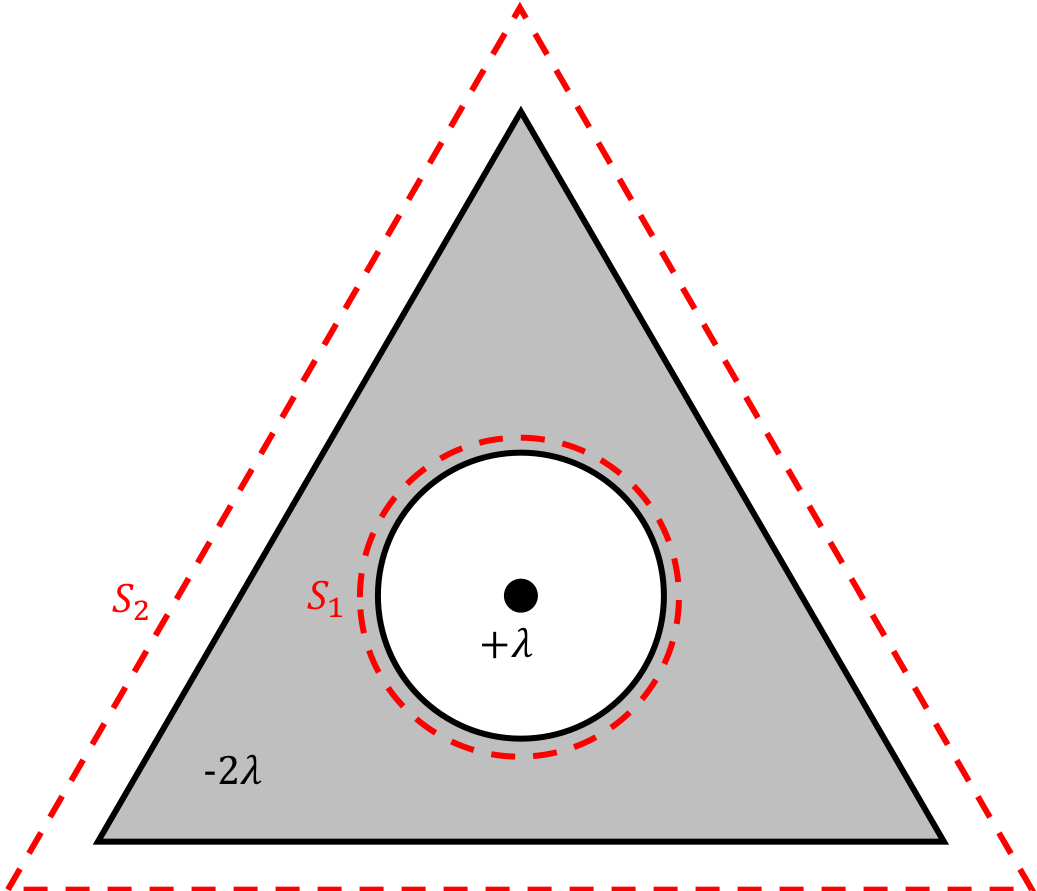
\includegraphics[width=0.4\linewidth]{files/coaxial_triangle_sid-52bfd62b5da7465dab59e3bae2b2561e.png}
\caption[]{Cross section of the wire/conducting shell set up, showing the Gaussian surfaces.}
\label{fig:gauss:coaxial_triangle_side}
\end{figure}
\end{framed}